 %  sample eprint article in LaTeX           --- M. Peskin, 9/7/00
%  modified for CTD2020, ctd2020-loc@iris-hep.org
%  This file is part of a tar file, which can be downloaded from the CTD2020 indico site. 
%  https://indico.cern.ch/event/742793/
%
\documentclass[10pt, paper=a4, UKenglish]{article}
\usepackage{graphicx}
\usepackage[utf8]{inputenc}
\usepackage{etoolbox,xspace}

% ...
% In this area
% The UTF-8 encoding is specified.
% ...
\inputencoding{latin1}
% ...
% Here the text encoding is specified as ISO Latin-1.
% ...
\inputencoding{utf8}
% Back to the UTF-8 encoding.
% ...
%
%%%%%%%%%%%%%%%%%%%%%%%%%%%%%%%%%%%%%%%%%%%%%%%%%%%%%%%%%%%%%%%%%%%%%%%%%%%%
%   document style macros
%%%%%%%%%%%%%%%%%%%%%%%%%%%%%%%%%%%%%%%%%%%%%%%%%%%%%%%%%%%%%%%%%%%%%%%%%%%%
\def\Title#1{\begin{center} {\Large #1 } \end{center}}
\def\Author#1{\begin{center}{ \sc #1} \end{center}}
\def\Address#1{\begin{center}{ \it #1} \end{center}}
\def\andauth{\begin{center}{and} \end{center}}
\def\submit#1{\begin{center}Submitted to {\sl #1} \end{center}}
\newcommand\pubblock{\rightline{\begin{tabular}{l} Proceedings of CTD 2020\\ \pubnumber\\
         \pubdate  \end{tabular}}}

\newenvironment{Abstract}{\begin{quotation} \begin{center} 
             \large ABSTRACT \end{center}\bigskip 
   \begin{center}\begin{large}}{\end{large}\end{center}\end{quotation}}

\newenvironment{Presented}{\begin{quotation} \begin{center} 
             PRESENTED AT\end{center}\bigskip 
      \begin{center}\begin{large}}{\end{large}\end{center} \end{quotation}}

\def\Acknowledgements{\bigskip  \bigskip \begin{center} \begin{large}
      \bf ACKNOWLEDGEMENTS \end{large}\end{center}}

%%%%%%%%%%%%%%%%%%%%%%%%%%%%%%%%%%%%%%%%%%%%%%%%%%%%%%%%%%%%%%%%%%%%%%%%%%%% 
%  personal abbreviations and macros
%    the following package contains macros used in this document:
\input econfmacros.tex
%%%%%%%%%%%%%%%%%%%%%%%%%%%%%%%%%%%%%%%%%%%%%%%%%%%%%%%%%%%%%%%%%%%%%%%%%%%

\textwidth=6.5in
\textheight=8.75in
\hoffset=-0.85in
\voffset=-0.6in

%%  DO NOT CHANGE anything above.

% include packages you will need
\usepackage{color}
\usepackage{lineno}
\usepackage{subfig}
\usepackage{hyperref}


%%%%%%%%%%%%%%%%%%%%%%%%%%%%%%%%%%%%%%%%%%%%%%%%%%%%%%%%%%%%%%%%%%%%
% basic data for the eprint:
%%%%%%%%%%%%%%%%%%%%%%%%%%%%%%%%%%%%%%%%%%%%%%%%%%%%%%%%%%%%%%%%%%%%

%% preprint number data:
% Please replace XX by your contribution number in indico (a number between 01 to 62)
\newcommand\pubnumber{PROC-CTD2020-XX}

%% date
\newcommand\pubdate{\today}

%%  Affiliation
\def\affiliation{
$^1$Cornell University, Ithaca, NY, USA 14853, \\
$^2$Fermi National Accelerator Laboratory, Batavia, IL, USA 60510\\
$^3$Princeton University, Princeton, NJ, USA 08544 \\
$^4$UC San Diego, La Jolla, CA, USA 92093 \\
$^5$University of Oregon, Eugene, OR, USA 97403
}

%% Acknowledge the support
\def\support{\footnote{Work supported by  XYZ Foundation}}

%%%%%%%%%%%%%%%%%%%%%%%%%%%%%%%%%%%%%%%%%%%%%%%%%%%%%%%%%%%%%%%%%%%%%%%%%%%% 

\newcommand{\conference}{Connecting the Dots Workshop (CTD 2020)\\
April 20-30, 2020}

\usepackage{fancyhdr}
\pagestyle{fancy}
\definecolor{mygrey}{RGB}{105,105,105}
\fancyhf{} % sets both header and footer to nothing
\renewcommand{\headrulewidth}{0pt}
% \fancyhead[R]{\fontsize{8}{9} \color{mygrey} \selectfont  CTD 2020 \\}
\fancyhead[C]{\fontsize{7}{8} \color{mygrey} \selectfont Connecting
  the Dots. April 20-30, 2020\\}
\fancyfoot[C]{\thepage}

%%%%%%%%%%%%%%%%%%%%%%%%%%%%%%%%%%%%%%%%%%%%%%%%%%%%%%%%%%%%%%%%%%%%

\begin{document}
\newcommand{\mkFit}{\textsc{mkFit}\xspace}

% uncomment the following line for adding line numbers
% \linenumbers

% large size for the first page
\large
\begin{titlepage}
\pubblock

%% Change the title, name, abstract
%% Title 
\vfill
\Title{Parallelizing the Unpacking and Clustering of Detector Data for Reconstruction of Charged Particle Tracks on Multi-core CPUs and Many-core GPUs}
\vfill

%  if you need to add the support use this, fill the \support definition above. 
%  \Author{FIRSTNAME LASTNAME \support}
\Author{Giuseppe Cerati$^{2}$, Peter Elmer$^{3}$, Brian Gravelle$^{5}$, Matti Kortelainen$^{2}$, 
Vyacheslav Krutelyov$^{4}$, Steven Lantz$^{1}$, Mario Masciovecchio$^{4}$, Kevin McDermott$^{1}$, Boyana Norris$^{5}$, Allison Reinsvold Hall$^{2}$, Micheal Reid$^{1}$, Daniel Riley$^{1}$, 
Matev\v{z} Tadel$^{4}$, Peter Wittich$^{1}$, Bei Wang$^{3}$, Frank W\"urthwein$^{4}$, and Avraham Yagil$^{4}$ }
\Address{\affiliation}
\vfill

\begin{Abstract}
Charged particle tracking is the most computationally intensive step of event reconstruction at LHC. Due to the computational cost, the current CMS online HLT only performs track reconstruction in detector regions of interest identified by the hardware trigger or other detector elements. We have made significant progress towards developing a parallelized and vectorized implementation of the combinatoric Kalman filter algorithm for track building that would allow efficient global reconstruction of the entire event within the projected online CPU budget. Global reconstruction necessarily entails the unpacking and clustering of the hit information from all the silicon strip tracker modules; however, currently only modules selected by the regional reconstruction are processed. Therefore, we have recently begun to investigate improving the efficiency of the unpacking and clustering steps.

Here we report results from parallelizing the unpacking and clustering steps of the raw data from the silicon strip modules so that all the required hit information for global reconstruction can be produced efficiently. Concurrency in events is enabled through nested OpenMP parallelism on CPU and CUDA streams on GPU. We show performance evaluations of the new unpacking and clustering algorithms on Intel Xeon and NVIDIA GPU architectures.
\end{Abstract}
\vfill

% DO NOT CHANGE!!!
\begin{Presented}
\conference
\end{Presented}
\vfill
\end{titlepage}
\def\thefootnote{\fnsymbol{footnote}}
\setcounter{footnote}{0}
%

% normal size for the rest
\normalsize 

%% Your paper should be entered below. 

\section{Introduction}
\label{intro}
The reconstruction of charged particle trajectories (tracking) is a pivotal element of the reconstruction chain in Compact Muon Solenoid (CMS)~\cite{Chatrchyan:2008aa} as it measures the direction and momentum of charged particles, which is then also used as input for nearly all high-level reconstruction algorithms: vertex reconstruction, b-tagging, lepton reconstruction, isolation jet and missing transverse momentum reconstruction. Tracking by far is the most time consuming step of event construction and its time scales poorly with the detector occupancy. This brings computing challenge in the upcoming upgrade of the accelerator from the Large Hadron Collider (HLC) to the High-Luminosity LHC (HL-HLC) where the instantaneous luminosity will increase by an order of magnitude due to the increased number of overlapping proton-proton collision (pileup, PU). 

To address this challenge, the parallel Kalman filter tracking project \mkFit was established in 2014 with the goal to enable efficient tracking on modern computing architecture. Over the last 6 years, we have made significant progress towards developing a parallelized and vectorized implementation of the combinatoric Kalman filter algorithm for tracking \cite{Cerati_2017,Cerati_2019,2019arXiv190611744C,2020arXiv200206295C}. This allows efficient global reconstruction of the entire event with projected online CPU budget. This also opens possibility to deploy \mkFit into CMS High Level Trigger (HLT), where performance requirement is particularly strict. The current goal is to test the algorithm online in Run 3 of the LHC. 

Global reconstruction necessarily entails the unpacking and clustering of the hit information from all silicon strip tracker modules. However, the current CMS HLT only performs track construction in detector regions of interests around the direction of leptons or jets. Therefore, we have recently begun to investigate improving the efficiency of the unpacking and clustering steps. This document highlights the latest development in enabling parallelization of unpacking and clustering on modern computing architectures. We start from a standalone version of the unpacker, which uses real raw data and calibration data, but simplified versions of many related CMSSW classes. 

\section{Parallelization}
\label{para}
The CMS silicon strip tracker (SST) are organized by Front End Drivers (FEDs). Each FED consists of 96 optical channels with 256 strips per channels~\cite{CMSTWiki}. In every CMS event, only the strips that are measured to be above a threshold are recorded. In zero suppression mode, the measured signal within a FED is stored like a variant of compressed spare row (CSR) format, where the channel and strip numbers correspond to the row and column numbers (Figure ~\ref{fig:SSTlayout}). Besides the event-based SST data, pre-measured calibration data, e.g., gain and noise value for each strip are packed also by channels. 

\begin{figure}[!htb]
  \centering
  % \includegraphics[height=2in]{picture}
  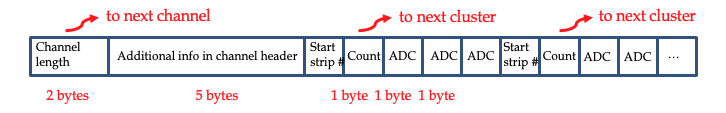
\includegraphics[scale=0.5]{SSTlayout}
  \caption{Raw data format from CMS SST}
  \label{fig:SSTlayout}
\end{figure}

Data layout is paramount to the performance, we therefore choose the structure-of-array (SoA) layout. The SoA approach maximizes spatial locality on streaming access and thus improves sustained bandwidth on both modern CPUs and GPUs. The unpacking step transforms all event-based SST data and pre-measured calibration data to the SoA format for providing optimal performance for the clustering step. Specifically, we constructs a map of the channel locations and attributes on CPU. The construction can only be done sequentially, but can overlap with raw data transfer. We then unpack the data to SoA format, which can be done concurrently for each channel. Unpacking is the most time consuming step since it involves irregular data access pattern and is particularly costly on GPU. 

The CMS clustering is based on the ``three thresholds" algorithm~\cite{CMSTWiki}. The parallel implementation is based on the fact that each candidate cluster will have at least one strip with signal to noise ratio larger than the ``seed threshold", which we call seed strips. We start from building an array of indices of seed strips. We then form candidate clusters by determining the left and right boundaries, compute the cluster charge and check it against the ``cluster threshold". Once passing ``three thresholds", we output its left and right boundaries, centroid and optionally ADC values for each cluster. The seed seeking stage can be parallelized over all strips and the cluster forming stage can be parallelized over all seed strips. 

\section{Optimization}
\label{opt}
In order to maximize the hardware usage and improve the overall throughput, we have enabled concurrency in processing multiple events. On CPU, this is achieved with OpenMP nested parallelism by creating two levels of OpenMP parallel regions, one inside the other. The outer level is used to handle different events while an inner level is used to handle sets of strips within a single event. To maintain good memory locality in nested parallelism, it is important to ensure that threads are given affinity to specific cores. It is also important that memory is placed locally to the processor that accesses the data. On GPU, we use CUDA streams to launch multiple events concurrently on the same device. This not only maximize GPU utilization, but also reduce data transfer overhead by overlapping communication with computation. We rely on the cached memory allocator developed as part of the PATATRACK project~\cite{PATATRACK} at CMSSW for GPU memory allocation. This has significantly reduce the memory allocation and deallocation overhead in processing multiple events. 

\section{Performance Results}
We evaluate the performance of the parallel implementation on Tigercpu, the GPU cluster at research computing of Princeton University. Each node in Tigercpu equips with two 2.4 GHz Xeon Broadwell E5-2680 v4 on the host and four 1328 MHz NVIDIA P100 GPU as accelerators. For CPU results, each test uses all 28 cores with nested parallelism. For GPU results, we use OpenMP to schedule multiple events concurrently on a single GPU. Table \ref{tab:perf} shows the wall-clock time and throughput results in running 840 events, where the same TTBar PU70 event data is used for all events. On CPU, the best performance is observed in running 14 events concurrently with 2 cores per event while on GPU running 2 events/streams concurrently results in the best performance. 

\begin{table}[!htb]
    \begin{minipage}{.5\linewidth}
      \centering
          \caption*{2x2.4 GHz Xeon Broadwell E5-2680 v4}    
          \begin{tabular}{c|cc}
      \hline
      \hline
      NxM & times (s) & throughput (events/s) \\
      \hline
      1x28 &  1.7 & 492  \\
      2x14 &   2.1 & 400  \\
      4x7 & 1.67 & 502 \\
      7x4 & 1.57 & 532 \\
      14x2 & 1.50 & 560 \\
      28x1 & 2.10 & 400 \\
      \hline
      \hline
    \end{tabular}
        \end{minipage}%
    \begin{minipage}{.5\linewidth}
      \centering
             \caption*{1238MHz NVIDIA P100}    
      \begin{tabular}{c|cc}
      \hline
      \hline
      N &  times (s) & throughput (events/s)  \\
      \hline
      1 & 1.36 & 615 \\
      2 & 1.29 & 649 \\
      4 & 1.41 & 595 \\
      7 & 1.46 & 574 \\
      14 & 1.53 & 548 \\
      28 & 1.54 & 546 \\
      \hline
      \hline
    \end{tabular}
        \end{minipage} 
     \caption{Performance comparison in running 840 TTBar PU70 events. N is the events concurrency and M is the CPU parallelization within one event. The reported number for each test is the average of 10 trials.}
     \label{tab:perf}
     \end{table}

\section{Conclusions}
We have enabled parallelization of unpacking and clustering and demonstrated its performance on both multi-core CPU and many-core GPU. Overall, we observe that GPU (P100) outperforms CPU(2x14 cores Broadwell) by 24\% in average. Next, we will integrate the implementation with CMSSW and convert clusters to global hit coordinates to provide as the input for \mkFit. 

%%%%%%%%%%%%%%%%%%%%%%%%%%%%%%%%%%%%%%%%%%%%%%%%%%%%%%%%%%%%%%%%%%%%%%%%%%%  

%%  if necessary
\Acknowledgements
This work is supported by the U.S. National Science Foundation, under grants PHY1520969, PHY1521042, PHY1520942 and PHY1624356, and under Cooperative Agreement OAC1836650, and by the U.S. Department
of Energy, Office of Science, Office of Advanced Scientific Computing Research, Scientific Discovery through Advanced Computing (SciDAC) program. This research used resources at research computing of Princeton University.
%%%%%%%%%%%%%%%%%%%%%%%%%%%%%%%%%%%%%%%%%%%%%%%%%%%%%%%%%%%%%%%%%%%%%%%%%%%

%\begin{thebibliography}{99}

%%
%%  bibliographic items can be constructed using the LaTeX format in SPIRES:
%%    see    
%%  SPIRES will also supply the CITATION line information; please include it.
%%

%\bibitem{example} 
 % Author 1,
 % "Article title,''
% Journal {\bf Volume}, Pages (Year)
 % [arXiv:XXXX.YYYY [ZZZZ]].

%\end{thebibliography}

\bibliographystyle{habbrv}
\bibliography{references}
%%%%%%%%%%%%%%%%%%%%%%%%%%%%%%%%%%%%%%%%%%%%%%%%%%%%%%%%%%%%%%%%%%%%%%%%%%%

\end{document}

